\section{BREVE INTRODUÇÃO AO CURSO}
Independente de sua cidade natal, de estar morando sozinho, com os pais ou até em uma república, nós sabemos o quão diferente é a vida acadêmica do colégio e do cursinho. Sempre é uma grande mudança e um grande passo para qualquer jovem, aqui nós damos algumas dicas sobre as matérias dos seus primeiros semestres e como funciona o sistema de requisitos de nosso curso.

Na UFSCar utilizamos o sistema de créditos - você pode entender créditos como horas semanais de um semestre - em que, no curso Ciência da Computação você precisará de 216 créditos para se formar sendo elas: 154 de disciplinas obrigatórias, 24 de optativas, 2 de eletivas, 24 do Trabalho de Graduação ou Estágio e 12 créditos de atividades complementares. Como aluno, é necessário que você complete pelo menos 8 créditos em um ciclo de um ano (contabilizando o semestre atual com o semestre anterior). Caso esse número de créditos não seja atingido, o estudante é considerado “jubilado” e sua matrícula é cancelada, perdendo a vaga. Além deste requisito, o calouro tem que passar em pelo menos 4 créditos no primeiro semestre para não perder a vaga. Isso pode ser reversível com a utilização do recurso (e é claro, uma justificativa convincente). Por isso muito cuidado!

O IRA é o Índice de Rendimento Acadêmico e é adotado para classificação na concorrência de prioridade de inscrição de disciplinas, transferências internas, bolsas para iniciação científica e até para programas externos como Ciência Sem Fronteiras. 

Abaixo temos um ilustrativo de como serão os três primeiros semestres dos ingressantes. As setas cheias representam quais matérias precisam ter aprovações para se cursar as outras, já as setas pontilhadas são aquelas que são recomendadas.

\begin{figure}[h]
    \centering
    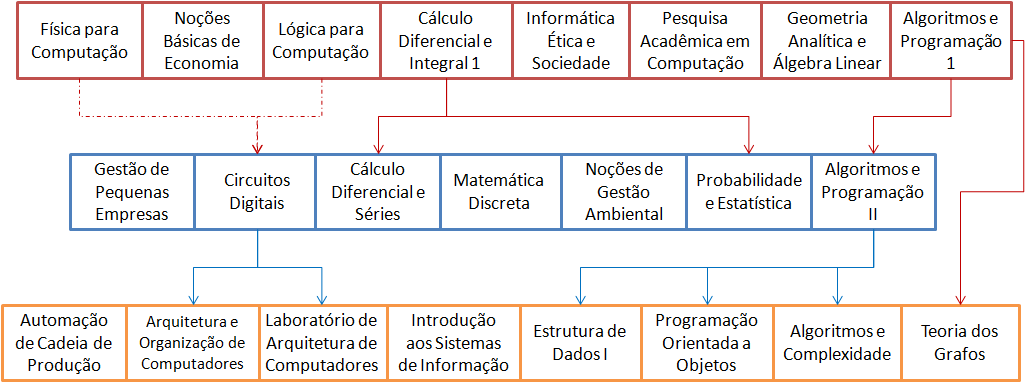
\includegraphics[width=\textwidth]{./imagem/requisitos_materias.png}
\end{figure}

O que acontece se você por acaso não passar em uma matéria? Ele fica com a famosa dependência ou DP, tendo de refazê-la em um semestre futuro. Note a importância de Algoritmos e Programação 1, por exemplo, cuja DP não permite cursar uma matéria no segundo semestre e quatro matérias no segundo, o que acaba atrasando um pouco o curso.
